% =====================================================================
% CHAPTER CONTENT BEGINS
% =====================================================================

\section{Empirical Equivalence of Factored L2 and Nuclear Norm Regularization in Asymmetric Burer-Monteiro Factorization}

\subsection{Introduction}
This story begins outside this experiment, in a different setting altogether. While exploring low-rank optimization and Burer-Monteiro (BM) factorization in the context of transformer architectures, we came across the recent work of Kobayashi, Akram, and von Oswald \cite{kobayashi2024lowrank}, which makes a deceptively simple observation about how weight decay interacts with the structure of attention layers.

The observation is the following. In a transformer attention layer, the effective weight matrix is not a single learned matrix $W$, but the product of two learned matrices $W = W_Q W_K^T$, where $W_Q$ and $W_K$ are the query and key projection matrices. When standard $L_2$ weight decay is applied to $W_Q$ and $W_K$ separately, as is the default in essentially every modern optimizer, something quietly happens that nobody had cleanly articulated before: this routine penalty is no longer a routine penalty. It becomes mathematically equivalent to nuclear norm regularization on the product $W_Q W_K^T$, which is the convex relaxation of rank itself. In other words, the standard training recipe is implicitly biasing the attention weights toward low rank, with no one having explicitly asked for that.

The authors prove this in two steps. First, they show that if $L_2$ regularization were applied directly to a single matrix $W$, with an objective of the form
\begin{equation}
    \mathcal{L}(W) = \mathcal{L}_{\text{data}}(W) + \frac{\lambda}{2} \|W\|_F^2,
\end{equation}
This shrinks $W$ uniformly and leaves its rank unchanged. The penalty has no opinion about rank in this form. Second, they show that the moment the same penalty is applied to a \textit{factorized} parameterization $W = UV^T$ with $U \in \mathbb{R}^{m \times k}$ and $V \in \mathbb{R}^{n \times k}$, the objective
\begin{equation}
\begin{aligned}
    \mathcal{L}(U, V) &= \mathcal{L}_{\text{data}}(UV^T) \\
    &\quad + \frac{\lambda}{2}\left(\|U\|_F^2 + \|V\|_F^2\right)
\end{aligned}
\end{equation}
is provably equivalent to the nuclear norm formulation
\begin{equation}
    \mathcal{L}_*(W) = \mathcal{L}_{\text{data}}(W) + \lambda \|W\|_*,
\end{equation}
where $\|\cdot\|_*$ denotes the nuclear norm. The equivalence rests on the classical Srebro-Shraibman variational identity \cite{srebroshraibman2005},
\begin{equation}
    \|W\|_* = \min_{U, V : UV^T = W} \frac{1}{2}\left(\|U\|_F^2 + \|V\|_F^2\right),
\end{equation}
which says the nuclear norm of $W$ is exactly the minimum of the factored $L_2$ objective over all factorizations $W = UV^T$. Theorem 3.3 of \cite{kobayashi2024lowrank} formalizes that the local minima of the factored objective coincide with those of the nuclear-norm one, and Theorem 3.4 strengthens this further by showing that during gradient flow training, the gap between the factored $L_2$ surrogate and the true nuclear norm decays exponentially fast. The decomposition itself, in short, is what creates the low-rank pressure, not the penalty form alone.

The natural next thought, and the one that motivates this section, was the following. The Burer-Monteiro factorization is not specific to transformers. It is the standard parameterization across an entire class of low-rank recovery problems: matrix completion, matrix sensing, low-rank matrix regression, recommender systems, and others. In all of these, the established regularizer is the same factored $L_2$ form $(\lambda/2)(\|U\|_F^2 + \|V\|_F^2)$. If the equivalence claimed by \cite{kobayashi2024lowrank} is real, then in any of these problems we should be able to replace the factored $L_2$ penalty with a direct nuclear norm penalty $\lambda \|UV^T\|_*$ and recover the same solution. This section sets up that comparison on the matrix sensing problem and tests it empirically.



\subsection{The Asymmetric BM Setting and the Question}
The asymmetric Burer-Monteiro factorization $W = UV^T$ is the canonical parameterization in a wide class of low-rank recovery problems, matrix completion, matrix sensing, low-rank matrix regression, and inductive matrix completion among them. In nearly all such problems, the established regularizer is the factored $L_2$ form $(\lambda/2)(\|U\|_F^2 + \|V\|_F^2)$, chosen for its smoothness and separability over $U$ and $V$. The nuclear norm $\|UV^T\|_*$, while theoretically the quantity of interest, is non-smooth and requires a singular value decomposition at each gradient step, making it computationally less attractive.

This raises a natural empirical question. If the factored $L_2$ formulation is mathematically equivalent to the nuclear norm formulation at the optimum, per the Srebro-Shraibman identity and Theorem 3.3 of \cite{kobayashi2024lowrank}, do the two penalties produce identical recovered matrices in practice? This section presents a controlled experiment to test this equivalence on the matrix sensing problem.

\subsection{Problem Statement: Matrix Sensing}
Matrix sensing is the canonical synthetic setting for low-rank recovery from linear measurements. An unknown matrix $M^* \in \mathbb{R}^{m \times n}$ of rank $r^*$ is observed only through $N$ scalar linear measurements
\begin{equation}
    y_i = \langle A_i, M^* \rangle, \quad i = 1, 2, \dots, N,
\end{equation}
where each $A_i \in \mathbb{R}^{m \times n}$ has entries drawn i.i.d.\ from $\mathcal{N}(0, 1/N)$. The Gaussian sensing ensemble satisfies the Restricted Isometry Property (RIP) with high probability when $N \gtrsim r^*(m+n)$. This condition guarantees the absence of spurious local minima in the BM landscape \cite{rechtfazelparrilo2010, tu2016procrustes}.

The true minimum-rank-recovery formulation,
\begin{equation}
    \min_{W} \text{rank}(W) \quad \text{subject to} \quad \langle A_i, W \rangle = y_i,
\end{equation}
is NP-hard. The standard convex relaxation replaces the rank with the nuclear norm. Adopting the unconstrained Lagrangian formulation and applying the asymmetric BM factorization $W = UV^T$ yields the optimization actually solved in practice:
\begin{equation}
\begin{aligned}
    \min_{U, V} \ &\frac{1}{2}\|\mathcal{A}(UV^T) - y\|_2^2 \\
    &+ \frac{\lambda}{2}\left(\|U\|_F^2 + \|V\|_F^2\right),
\end{aligned}
    \label{eq:bm_l2}
\end{equation}
where $\mathcal{A}: \mathbb{R}^{m \times n} \to \mathbb{R}^N$ denotes the linear measurement operator with $[\mathcal{A}(W)]_i = \langle A_i, W \rangle$. Equation (\ref{eq:bm_l2}) is the standard formulation in the matrix-sensing literature.

\subsubsection{The Two Variants Under Comparison}
We compare Equation (\ref{eq:bm_l2}) against an alternative formulation in which the factored $L_2$ penalty is replaced by a direct nuclear norm penalty on the product:
\begin{equation}
    \min_{U, V} \ \frac{1}{2}\|\mathcal{A}(UV^T) - y\|_2^2 + \lambda \|UV^T\|_*.
    \label{eq:bm_nuc}
\end{equation}
The data fidelity term and the regularization strength $\lambda$ are held identical. Only the penalty form differs.

\subsection{Hypothesis}
We hypothesize that the nuclear norm formulation, Equation (\ref{eq:bm_nuc}), will recover a matrix of rank \textit{less than or equal to} that recovered by the factored $L_2$ formulation, Equation (\ref{eq:bm_l2}). The intuition behind this is that the nuclear norm acts directly on the product $UV^T$, which is the quantity whose rank we care about, whereas the factored $L_2$ penalty acts on $U$ and $V$ separately and is only an upper bound on the nuclear norm during training, tight only at convergence. If the nuclear norm penalty is more aggressive or more direct in pruning singular values, this would show up as a strictly lower or equal  recovered rank to the one of L2 penalty. Theorem 3.3 of \cite{kobayashi2024lowrank} predicts the two ranks should in fact be equal at convergence, which would mean the factored $L_2$ penalty is a tight surrogate, not just an upper bound. The experiment will tell us which is the case.

\subsection{Methodology}

\subsubsection{Problem Generation}
For each experimental cell, the ground truth matrix $M^* \in \mathbb{R}^{m \times n}$ was constructed as $M^* = U^* (V^*)^T$ with $U^* \in \mathbb{R}^{m \times r^*}$ and $V^* \in \mathbb{R}^{n \times r^*}$ having entries drawn i.i.d.\ from $\mathcal{N}(0, 1)$, then rescaled so that $\|M^*\|_F = 1$. This normalization keeps the matrix size constant across all values of $r^*$, so any differences observed across the rank sweep can be attributed to rank alone and not to changes in matrix scale. .

The sensing operator was instantiated as a tensor of shape $(N, m, n)$ with each $A_i$ having entries i.i.d.\ from $\mathcal{N}(0, 1/N)$. The measurement vector $y \in \mathbb{R}^N$ was computed as $y_i = \langle A_i, M^* \rangle$ in the noiseless regime.

\subsubsection{Optimization Setup}
The BM factor matrices $U \in \mathbb{R}^{m \times k}$ and $V \in \mathbb{R}^{n \times k}$ were initialized with entries i.i.d.\ from $\mathcal{N}(0, 0.01^2)$. Optimization used the Adam optimizer with learning rate $10^{-3}$, $\beta_1 = 0.9$, $\beta_2 = 0.999$, and decoupled weight decay set to zero (the regularization is included explicitly in the objective). A maximum budget of $10{,}000$ gradient steps was allowed per run, with early stopping triggered when the variation in the total loss over the trailing window of $100$ steps fell below $10^{-8}$.


\subsubsection{Experimental Grid and Pairing}
The first phase swept the true rank $r^* \in \{2, 3, 5, 8\}$. The remaining knobs were tied to $r^*$: the BM inner width $k = 2r^*$ (overcomplete) and the number of measurements $N = 5 r^* (m + n)$, well above the RIP threshold. The matrix dimensions were fixed at $(m, n) = (100, 100)$, the regularization strength at $\lambda = 0.1$, and the noise level at $\sigma = 0$ throughout. Three independent seeds were run per cell.

A critical design choice for the comparison was paired execution: within each $(r^*, \text{seed})$ cell, both the $L_2$ and the nuclear norm runs used the same $M^*$, the same sensing operator $A$, and the same initialization $(U_0, V_0)$. The only variable was the penalty form. This isolates the regularizer's effect from sample-level randomness in the comparison.

\subsubsection{Metrics}
At the conclusion of each run, we computed the singular values of the recovered matrix $W = UV^T$ and reported two complementary rank estimates:
\begin{itemize}
    \item \textbf{Effective Rank:} the number of singular values exceeding $0.01 \cdot \sigma_{\max}$, where $\sigma_{\max}$ is the largest singular value. This thresholded count is robust to floating-point noise floors.
    \item \textbf{Pseudo-Rank:} the smallest $k$ such that the cumulative sum of the top-$k$ singular values exceeds $95\%$ of the total spectral mass.
\end{itemize}


\subsection{Results and Discussion}
The Phase 1 sweep produced $24$ runs ($4$ values of $r^*$ $\times$ $3$ seeds $\times$ $2$ penalties). Across all cells, the recovery succeeded and the comparison between the two penalty forms is decisive.

\subsubsection{Rank Recovery and Penalty Equivalence}
Figure \ref{fig:pseudo_rank} plots the pseudo-rank against the true rank $r^*$ for both penalties. The two curves overlap exactly with the diagonal $y = r^*$ at every value of $r^*$ tested. The effective rank, plotted on the same axes, is identical to the pseudo-rank in every cell, a consequence of the spectral cliff described below. The recovered rank lies far below the search-space ceiling $k = 2r^*$, confirming that the regularizer is performing genuine pruning rather than passively saturating the available BM width.

\begin{figure}[htbp]
  \centering
  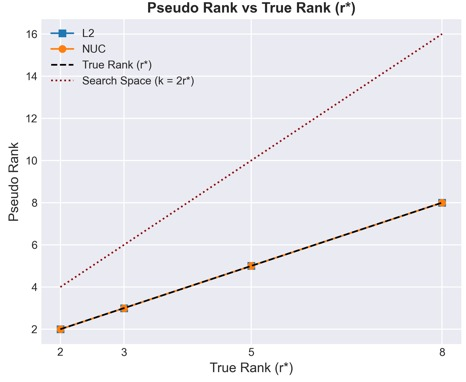
\includegraphics[width=\columnwidth]{pic1.jpeg}
  \caption{Both penalties recover rank exactly equal to $r^*$ across all tested values, with the search-space ceiling $k = 2r^*$ shown as reference.}
  \label{fig:pseudo_rank}
\end{figure}

The singular value spectra (Figure \ref{fig:svd_spectrum}) make the equivalence visually unambiguous. In every panel, the recovered matrix exhibits a sharp cliff at index $r^*$, with kept singular values of magnitude $\mathcal{O}(0.1)$ to $\mathcal{O}(1)$ and pruned singular values sitting at the optimizer's noise floor of approximately $10^{-7}$. The drop spans six to seven orders of magnitude, leaving no ambiguity about the recovered rank. The $L_2$ and nuclear norm spectra coincide throughout, kept singular values, noise floor, and the slope of the spectrum within the kept block are all visually indistinguishable. The two penalties do not merely produce the same rank; they produce essentially the same matrix $W$.

\begin{figure}[htbp]
  \centering
  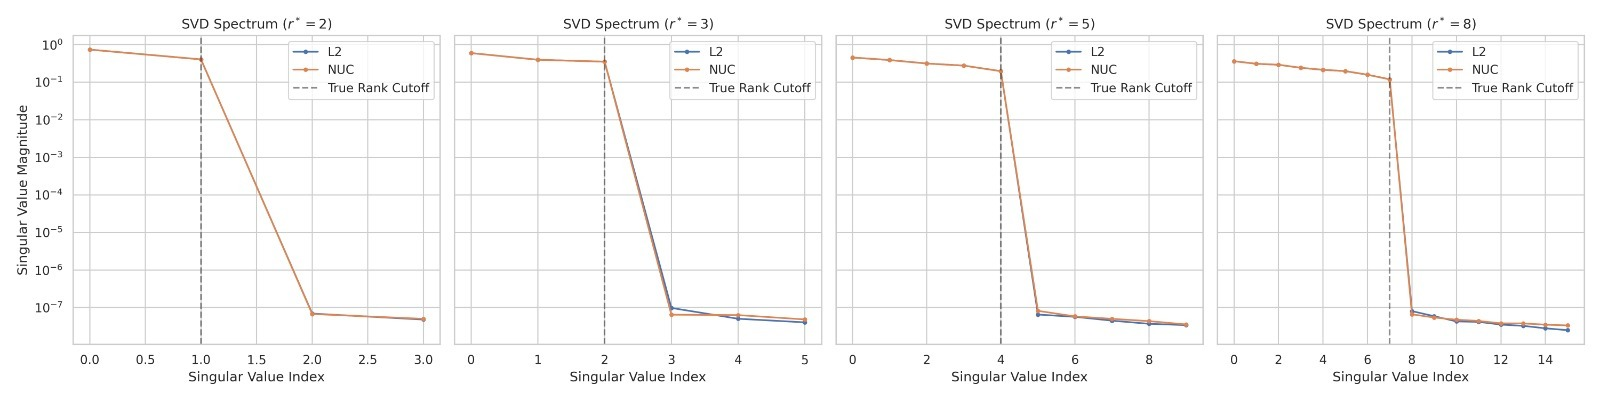
\includegraphics[width=\columnwidth]{pic2.jpeg}
  \caption{Singular values of $W = UV^T$ at convergence, log scale. The cliff at index $r^*$ separates kept singular values ($\mathcal{O}(0.1)$ to $\mathcal{O}(1)$) from pruned ones ($\mathcal{O}(10^{-7})$). $L_2$ and nuclear norm curves overlap.}
  \label{fig:svd_spectrum}
\end{figure}
These results confirm Hypothesis H1: the factored $L_2$ and direct nuclear norm penalties on the asymmetric BM factorization produce identical recovered solutions in the matrix sensing setting. Theorem 3.3 of \cite{kobayashi2024lowrank} is verified empirically across the rank sweep.

\subsubsection{Iteration Cost: A Practical Asymmetry}
While the two penalties agree at the optimum, they differ sharply in the number of gradient steps required to reach it. Figure \ref{fig:iters} plots the iteration count against $r^*$ for each penalty. The $L_2$ runs early-stop at approximately $1{,}500$ steps for $r^* \in \{2, 3\}$ and around $4{,}000$ steps for $r^* \in \{5, 8\}$. The nuclear norm runs, in contrast, exhaust the full $10{,}000$-step budget in every cell.

\begin{figure}[htbp]
  \centering
  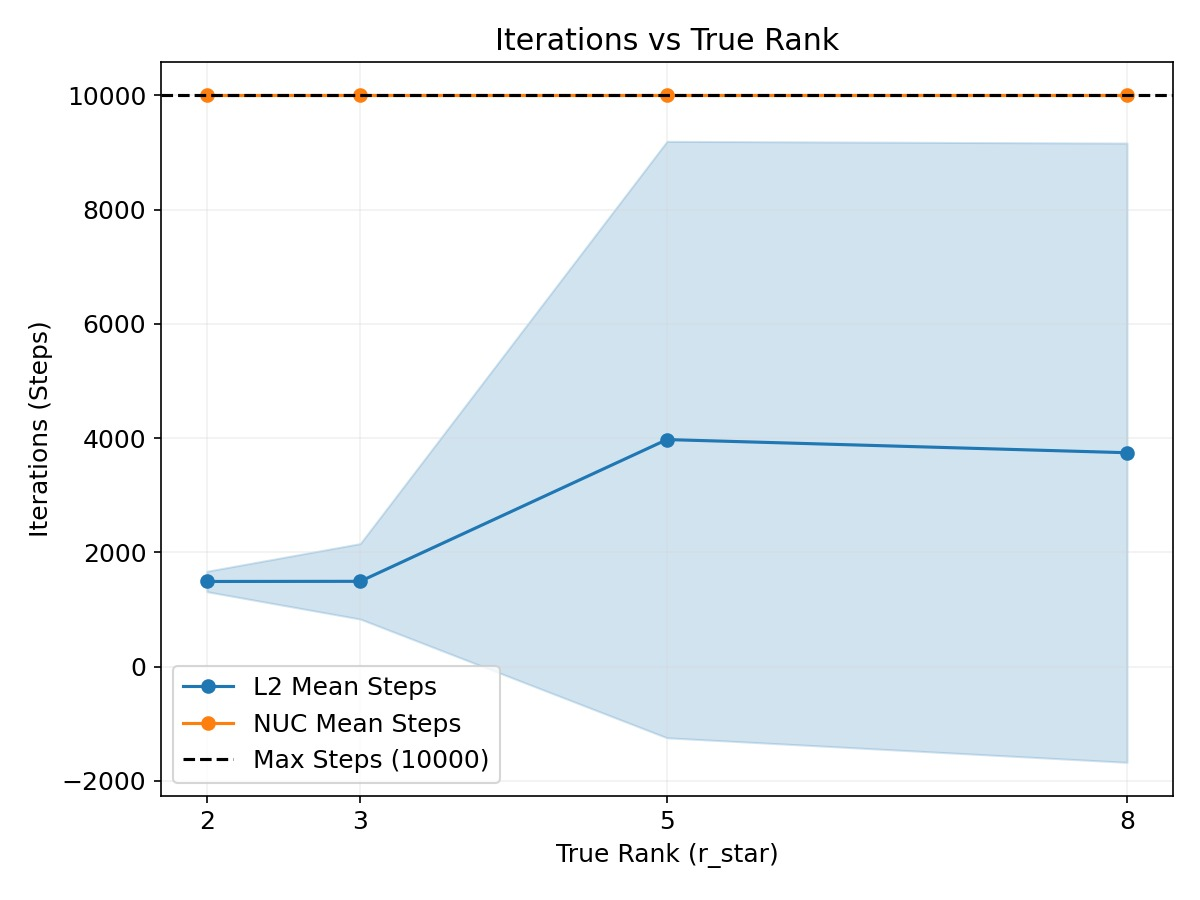
\includegraphics[width=\columnwidth]{pic3.jpeg}
  \caption{The $L_2$ runs converge under the early-stopping criterion well before the iteration budget is exhausted. The nuclear norm runs reach the maximum step count in every cell.}
  \label{fig:iters}
\end{figure}

\subsubsection{Why the Iteration Cost Diverges}
The asymmetry has a clean explanation rooted in the structure of the two penalties:

\begin{itemize}
    \item \textbf{The $L_2$ penalty is smooth and separable.} The term $(\lambda/2)(\|U\|_F^2 + \|V\|_F^2)$ decomposes elementwise over the entries of $U$ and $V$, with gradient $\lambda U$ and $\lambda V$ respectively. Each gradient step is computationally trivial and well-conditioned, and the loss surface admits rapid convergence under Adam.
    \item \textbf{The nuclear norm penalty is non-smooth.} The term $\lambda \|UV^T\|_*$ requires a full singular value decomposition of the product $UV^T$ at every gradient step in order to compute the penalty value and its gradient. The backward pass through the SVD involves operations on the full matrix of singular vectors, coupling all entries of $U$ and $V$ through a non-smooth function. Even after the rank has stabilized, the optimizer continues to register non-trivial gradient signal and does not satisfy the early-stopping criterion within the allotted budget.

\end{itemize}

This iteration-and-cost gap is precisely the practical reason the BM literature has uniformly settled on the factored $L_2$ formulation. The Srebro-Shraibman identity guarantees that $L_2$ on the factors is a faithful surrogate for nuclear norm regularization on the product, and the surrogate happens to be both smooth and decoupled. The non-smooth original is a worse computational choice for an identical statistical outcome.

\subsection{Conclusion}
This experiment provides a controlled empirical confirmation that, in the asymmetric Burer-Monteiro setting on a matrix sensing problem, the factored $L_2$ and direct nuclear norm regularizers converge to identical solutions. The recovered rank, the singular value spectrum, and the reconstruction error coincide between the two formulations across the swept range of true ranks. Theorem 3.3 of \cite{kobayashi2024lowrank} is verified outside the transformer attention setting in which it was originally developed.

The experiment additionally surfaces a practical asymmetry: the nuclear norm formulation, while statistically equivalent, is substantially more expensive per gradient step due to the SVD it requires, and exhibits delayed convergence behavior under standard early stopping. This documents quantitatively the implicit cost-benefit calculation that underlies the dominance of the factored $L_2$ formulation in the matrix completion, matrix sensing, and recommender systems literature.

Subsequent phases of this study extend the rank sweep to $r^* \in \{10, 15, 20\}$, vary the regularization strength $\lambda$ to map the rank-pruning transition, and investigate whether the equivalence persists under noise and incomplete observation regimes.
